\section{LLM 推理与服务}
\label{sec:infer}

2023 年以来，LLM 推理是面试中权重上升最快的方向。它和训练最大的区别在于自回归的 decode：每生成一个 token，都要把全部权重和这条序列的全部 KV cache 读一遍，
计算量却只有 $2N$ FLOPs。所以推理的很多问题，归根到底是「每生成一个 token 要读多少字节」的问题。本节先用 roofline 区分 prefill 和 decode，再推导 KV cache 的大小，
然后讨论批处理与调度（continuous batching、PagedAttention、chunked prefill、PD 分离、前缀缓存），最后是推测解码和量化。

\subsection{Prefill 与 decode 的 roofline}

一次请求分两个阶段。prefill 一次处理整段 prompt，线性层是 $[B\cdot T_p, d]\times[d,d]$ 的 GEMM，强度很高，受算力限制，它决定了首 token 时延（TTFT）。
decode 每步每条序列只处理一个 token，线性层退化成 GEMV（batch 为 $B$ 时是 $M=B$ 的瘦 GEMM），受带宽限制，它决定了每 token 时延（TPOT）。
Pope 等人对此做过系统的分析~\cite{pope2023efficiently}。忽略非矩阵运算，一个 decode 步的 roofline 下界是
\begin{equation}
t_{\text{dec}} \approx \max\!\left(\frac{2NB + 4Ld\,TB}{P_{\text{peak}}},\ \frac{sN + \mathrm{KV}(T,B)}{\mathrm{BW}}\right),
\label{eq:decode}
\end{equation}
其中 $4LdTB$ 是 attention 对长度为 $T$ 的上下文做点积和加权求和的运算量，$\mathrm{KV}(T,B)$ 是 KV cache 的字节数（式~\eqref{eq:kv}）。
如果只看权重，强度 $I\approx2NB/(sN)=B$（BF16），也就是说\emph{临界 batch 约等于拐点}，H100 上 $B^\ast\approx295$。
但 KV 的读取不能被 batch 分摊，每条序列都要读自己的 KV，所以长上下文下它会先成为瓶颈。
图~\ref{fig:intbatch} 显示了这一点：上下文为 4096 时，Llama-3-8B 的 decode 强度在大 batch 下趋于约 30；上下文到 32K 时只有约 7，永远到不了拐点。
相比之下，prefill（每条序列 512 token）的线性层强度在 batch 1 时就已经超过 400。

\begin{figure}[!t]
\centering
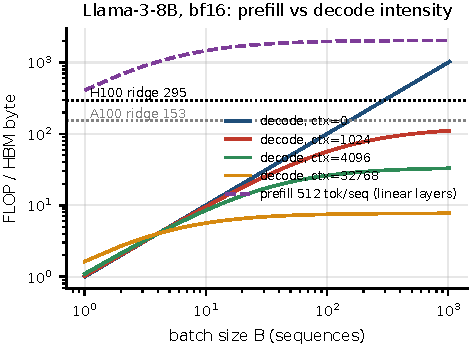
\includegraphics[width=\columnwidth]{fig_intensity_batch}
\caption{Llama-3-8B 在 BF16 下 prefill 与 decode 的算术强度随 batch 的变化（\texttt{mlsys\_calc.decode\_step\_time}）。
不计 KV（ctx=0）时，decode 强度等于 $B$，在 $B\approx295$ 处越过 H100 的拐点；计入 KV 后，强度会饱和在一个由上下文长度决定的常数上，
因为 KV 字节随 batch 同步增长。prefill 的线性层在任何 batch 下都受算力限制。}
\label{fig:intbatch}
\end{figure}

强度饱和意味着吞吐也会饱和。图~\ref{fig:decodetput} 把强度换算成了 decode 吞吐的上界。

\begin{figure*}[!t]
\centering
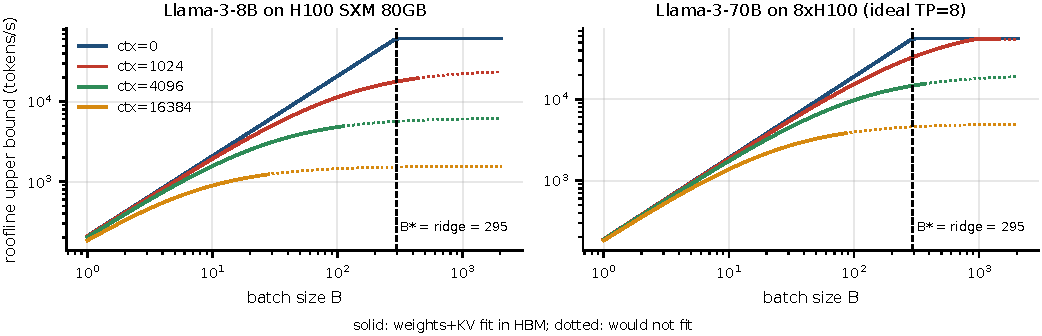
\includegraphics[width=\textwidth]{fig_decode_throughput}
\caption{decode 吞吐的 roofline 上界随 batch 的变化。左：Llama-3-8B，单张 H100；右：Llama-3-70B，理想 TP=8 的 8 卡 H100（聚合算力与带宽，忽略 all-reduce）。
实线表示权重和 KV 能放进 HBM，虚线表示放不下。ctx=0 的曲线在 $B^\ast=295$ 处出现从访存受限到算力受限的拐点；
上下文越长，曲线越早饱和，而且还没到拐点就因为 KV 放不下而终止。也就是说，长上下文下限制吞吐的是 KV 的带宽和容量，而不是算力。}
\label{fig:decodetput}
\end{figure*}

\begin{est}{H100 上 Llama-3-8B 的 decode 上限}
权重 $8.03\times10^9\times2\approx16.06$~GB。batch=1、上下文 4096 时，KV 是 0.54~GB，每步读 16.6~GB，$t\ge16.6/3.35\approx4.95$~ms，约 202~token/s；
而计算只有 $2N\approx16$~GFLOP，只用到峰值的 0.3\%。batch=64 时，KV 是 34.4~GB，每步 15.05~ms，约 4252~token/s，仍然受访存限制。
batch=256 时，KV 达到 137~GB，单卡放不下（\texttt{inference\_math.csv} 与配套实验 CS229S P2 一致）。
作为对比，看短上下文的 7B 模型在 batch=512 时的情况：读权重 14~GB 需要 4.2~ms，计算 $2\times7\times10^9\times512/989\times10^{12}\approx7.2$~ms，
\emph{已经受算力限制}了。RL rollout 这类大 batch 场景里推测解码收益消失，原因就在这里。
\end{est}

\begin{qa}{prefill 和 decode 的瓶颈分别是什么？这对系统设计意味着什么？}
\ans prefill 是 GEMM，受算力限制，决定 TTFT 和算力需求；decode 是 GEMV 或瘦 GEMM，受带宽限制，因为要读全部权重和 KV，它决定 TPOT 以及对显存带宽和容量的需求。
两者混在一起跑会互相干扰：一个长 prefill 会让同批 decode 的 TPOT 抖动。由此引出了两种设计：chunked prefill 把 prefill 切块混进 decode 步；
PD 分离把两者部署到不同的池子里，各自按 TTFT 和 TPOT 选择并行度。
\wrong 「decode 慢是因为计算量大」。
\end{qa}

\subsection{KV cache 的大小}

既然 KV 会成为瓶颈，就得会算它有多大。每一层、每个 token 都要存一个 K 向量和一个 V 向量，长度都是 $n_{kv}\cdot d_{\text{head}}$，所以
\begin{equation}
\mathrm{KV}(T,B) = 2\cdot L\cdot n_{kv}\cdot d_{\text{head}}\cdot T\cdot B\cdot s .
\label{eq:kv}
\end{equation}
代入几个常见模型：Llama-3-8B（$L=32$、$n_{kv}=8$、$d_{\text{head}}=128$）是 128~KiB/token；Llama-3-70B（$L=80$、$n_{kv}=8$）是 320~KiB/token；
没有用 GQA 的 Llama-2-7B（$n_{kv}=32$）是 512~KiB/token~\cite{touvron2023llama,dubey2024llama3}。不同上下文长度下的数值见表~\ref{tab:kv} 和图~\ref{fig:kv}。

\begin{table}[!t]
\centering
\caption{KV cache 大小（BF16，batch=1，单位 GiB；\texttt{mlsys\_calc.kv\_cache\_bytes}）}
\label{tab:kv}
\footnotesize
\setlength{\tabcolsep}{4pt}
\begin{tabularx}{\columnwidth}{@{}l c c Y Y Y@{}}
\toprule
模型 & $n_{kv}$ & KiB/tok & 8K & 32K & 128K \\
\midrule
Llama-2-7B（MHA） & 32 & 512 & 4.0 & 16.0 & 64.0 \\
Llama-3-8B（GQA-8） & 8 & 128 & 1.0 & 4.0 & 16.0 \\
Llama-3-70B（GQA-8） & 8 & 320 & 2.5 & 10.0 & 40.0 \\
70B 若为 MHA（反事实） & 64 & 2560 & 20.0 & 80.0 & 320.0 \\
\bottomrule
\end{tabularx}
\end{table}

\begin{figure}[!t]
\centering
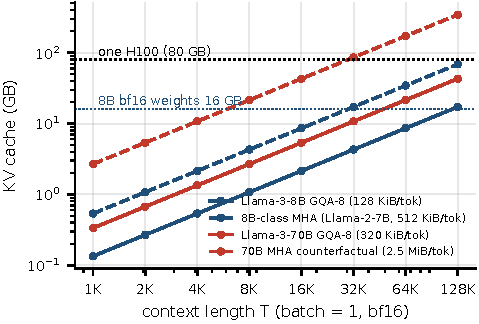
\includegraphics[width=\columnwidth]{fig_kv_cache}
\caption{KV cache 随上下文长度的增长（batch=1，BF16）。实线是采用 GQA-8 的真实模型，虚线是同规模的 MHA。
Llama-3-8B 在 128K 时 KV 为 16~GiB，已经和它 16~GB 的权重相当；70B 如果是 MHA，32K 上下文的一条序列就要 80~GiB，占满一张 H100。
GQA 把 KV 缩小了 $n_{\text{heads}}/n_{kv}$ 倍（8B 是 4 倍，70B 是 8 倍），同样的显存因此能放下长得多的上下文。}
\label{fig:kv}
\end{figure}

\begin{est}{8K 与 128K 上下文的 KV cache}
Llama-3-8B：$2\times32\times8\times128\times2=131072$~B=128~KiB/token。8K 的一条序列是 1~GiB，batch 32 是 32~GiB（34~GB）；128K 的一条序列是 16~GiB。
Llama-3-70B：320~KiB/token，8K 是 2.5~GiB，128K 是 40~GiB，一条 128K 的序列就要占半张 H100。同样条件下，Llama-2-7B 在 8K、batch 32 时需要 128~GiB。
到了 128K，decode 的瓶颈已经从「读权重」变成「读 KV」。KV 量化、GQA/MLA 和上下文并行都是从这里出发的。
\end{est}

\begin{qa}{KV cache 为什么能省计算？它本身的代价是什么？}
\ans 它省掉的是对前缀的重复计算。不缓存时，每一步都要为全部前缀重算 K、V 投影，生成 $T$ 个 token 总共要 $O(T^2)$ 次线性层；缓存之后每步只算新 token，总共 $O(T)$。
配套实验（CS229S P2，CPU）中，$T=1024$ 时 KV cache 把生成速度从 38.9 提到 499~token/s，快了 12.8 倍，总耗时也从 $\sim T^2$ 变成了 $\sim T$。
代价是显存 $2Ln_{kv}d_{\text{head}}TBs$，它决定了最大并发和最长上下文；而且每一步仍要读全部 KV 做点积，attention 的读取量随 $T$ 线性增长。
\wrong 「KV cache 减少了 attention 的计算」；或者计算 KV 大小时用了 $n_{\text{heads}}$ 而不是 $n_{kv}$（GQA 下会差 4--8 倍）。
\end{qa}

\subsection{MQA、GQA 与 MLA}

既然 KV 的大小正比于 $n_{kv}$，最直接的办法就是减少 KV 头。MQA~\cite{shazeer2019fast} 让所有查询头共享一组 K/V，KV 缩小 $n_{\text{heads}}$ 倍，但有质量损失。
GQA~\cite{ainslie2023gqa} 是折中：每组查询头共享一组 K/V，在质量和 KV 大小之间取平衡，而且可以从 MHA 的 checkpoint 经过少量 uptraining 得到。
二者都不改变 attention 的 FLOPs，因为每个查询头仍要和 $T$ 个 key 做点积；它们减少的是 KV 的存储和读取，所以 decode attention 的强度提高了 $n_{\text{heads}}/n_{kv}$ 倍。
DeepSeek-V2 的 MLA~\cite{deepseekai2024v2} 走得更远：它缓存一个低秩压缩的 latent（512 维）加一个解耦的 RoPE key（64 维），推理时把上投影矩阵吸收进查询和输出投影。
论文报告其 KV cache 比 DeepSeek 67B 减少了 93.3\%。

\begin{qa}{GQA、MLA、KV INT8 量化各自省了什么、代价是什么？}
\ans 三者都在减少 KV 的字节，方式不同，而且可以叠加。GQA 减少 KV 头数，KV 和 decode attention 的读取量都减少 $n_{\text{heads}}/n_{kv}$ 倍；它改变了模型结构，需要从训练开始用，或者做 uptraining。
MLA 缓存低秩 latent，压缩比更高，但实现复杂：RoPE 要解耦，还需要能吸收投影矩阵的 kernel。KV INT8/FP8 量化不需要重训，KV 直接减半，代价是轻微的精度损失和反量化开销。
\wrong 「GQA 减少了 attention 的 FLOPs」。
\end{qa}

\subsection{批处理与调度}

decode 受带宽限制，提高吞吐最有效的办法就是把更多请求拼进同一个 batch，让一次权重读取服务更多 token。下面五项技术都在回答同一个问题：怎样在显存和时延约束下把 batch 做大、做稳。

第一项是 continuous batching。传统的静态批处理要等一批里最长的请求生成完，才能换下一批。Orca~\cite{yu2022orca} 提出了 iteration-level 调度：
每个 decode 步都可以让完成的请求离开、让新请求加入；同时用 selective batching，只对线性层拼批，attention 则按请求分别计算。

第二项是 PagedAttention。如果按最大长度给每条序列连续预分配 KV，会产生大量内部碎片和预留浪费。vLLM~\cite{kwon2023vllm} 借鉴了操作系统的分页机制：
KV 按固定大小的块分配（默认 16 个 token 一块），用块表把逻辑块映射到物理块，浪费只发生在最后一块；并行采样和 beam search 还可以通过引用计数和 copy-on-write 共享前缀块。
论文报告的吞吐比当时的系统高 2--4 倍。

第三项是 chunked prefill。Sarathi-Serve~\cite{agrawal2024sarathi,agrawal2023sarathi} 把长 prompt 切成固定预算的块，和 decode 拼在同一步里执行（stall-free batching）。
decode 本来就受访存限制，捎带进去的 prefill 计算几乎是免费的；同时，长 prefill 再也不会让 decode「卡顿」。

第四项是 PD 分离。DistServe~\cite{zhong2024distserve} 和 Splitwise~\cite{patel2024splitwise} 把 prefill 和 decode 放到不同的 GPU 池里，各自选择并行度和 batch，
目标是优化 goodput，即满足 TTFT 和 TPOT 两个 SLO 的请求率。代价是 KV 需要跨卡甚至跨机传输。DistServe 报告，在相同 SLO 下可服务的请求率最高提升了 7.4 倍。

第五项是前缀缓存。SGLang~\cite{zheng2024sglang} 的 RadixAttention 用基数树管理 KV，自动复用不同请求之间共享的前缀，比如系统提示词、few-shot 示例和多轮对话历史；
它还配合缓存感知的调度，优先调度命中前缀较长的请求。

\begin{figure*}[!t]
\centering
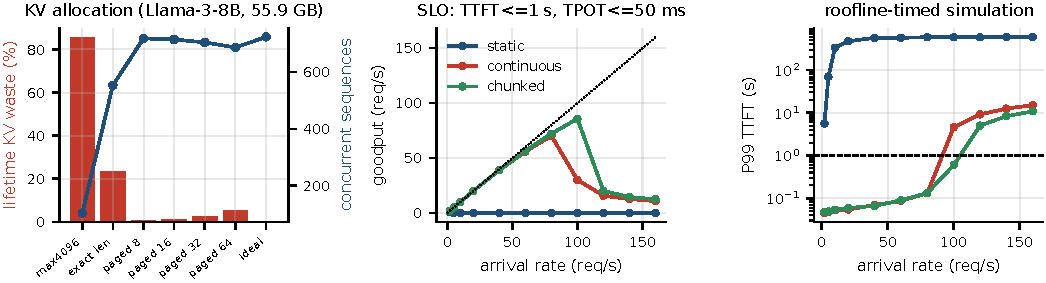
\includegraphics[width=\textwidth]{fig_lab_serving}
\caption{本文配套实验（15-849 服务与显存）中 KV 分配与调度的模拟结果（Llama-3-8B、H100，每步耗时取自 roofline 模型）。
左：10k 个请求（长度服从对数正态分布）在生命周期内的平均 KV 浪费和并发序列数。按 4096 连续预留时浪费 85.6\%、并发 104；即使预先知道最终长度也浪费 23.5\%；分页（block=16）只浪费 1.25\%，并发升到 714。
中：goodput 随到达率的变化（SLO 为 TTFT$\le$1~s 且 TPOT$\le$50~ms），static 的峰值是 0.97~req/s，continuous 是 70.2，chunked 是 85.7。
右：P99 TTFT，虚线是 1~s 的 SLO。所有时延都是模型输出，没有计入 kernel launch 和 CPU 调度开销，绝对值偏乐观；可以引用的是三者的相对关系和拐点位置。}
\label{fig:labserving}
\end{figure*}

这些机制的效果有多大？\lab{15-849 服务与显存}实现了块表、引用计数、copy-on-write fork、swap/recompute 两种抢占方式，以及按块表 gather 的 attention
（结果与连续存储的实现逐元素相等），再用离散事件模拟比较了三种调度（图~\ref{fig:labserving}）。
在饱和负载（$\lambda=160$~req/s）下，吞吐从 static 的 891~token/s 提到 continuous 的 14,050，再到 chunked 的 16,156。
最长的单次迭代从 5448~ms 降到 121~ms，再降到 9.2~ms；$\lambda=100$ 时，三者的 P99 TTFT 分别是 583~s、4.58~s 和 0.595~s。
显存紧张时差别更明显：把 KV 预算压到 6.55~GB、$\lambda=60$ 时，continuous 抢占了 73 次，重算了 26,480 个 prefill token，goodput 跌到 6.9~req/s；
chunked 只抢占了 39 次，goodput 保住了 51.1。分页的浪费也可以在白板上估出来：每条序列最多浪费 block$-1$ 个 token，平均约 block/2，
$8/590\approx1.4\%$，和实测的 1.25\% 吻合。

\begin{qa}{PagedAttention 解决的是什么问题？代价呢？block 大小怎么取？}
\ans 它解决的是 KV 的内部碎片和预留浪费，并没有让 KV 变小。按最大长度连续预留时，平均浪费可以超过 80\%；分页之后浪费只出现在最后一块，还能在并行采样、beam search 和共享前缀之间共用块。
代价是 attention kernel 要按块表间接寻址：块越小，访存越零碎，块表也越大；但块越小，浪费也越少。vLLM 默认取 16，是在浪费和 kernel 效率之间的折中。
\wrong 「PagedAttention 减少了 KV 的大小」。它减少的是浪费，不是 KV 本身。
\end{qa}

\begin{qa}{continuous batching 与 static batching 的区别？chunked prefill 又解决了什么？}
\ans 区别在于组批的时机。static batching 下，一批请求要等最长的那条结束，短请求空等，新请求排队；continuous batching 在每个 decode 步重新组批，吞吐和平均时延都更好。
但它留下了一个问题：新请求的整段 prefill 混进某一步时，这一步会变得很长，同批 decode 的 TPOT 出现明显的尖峰。chunked prefill 给每一步设一个 token 预算，把 prefill 切成块，
本文的模拟中最长的一步因此从 121~ms 降到了 9.2~ms。
\wrong 「continuous batching 就是 batch 更大」。
\end{qa}

\begin{qa}{chunked prefill 和 PD 分离怎么选？}
\ans 看规模和 SLO。chunked prefill 在同一组 GPU 上平滑干扰，部署简单，也不用传 KV，但 prefill 和 decode 只能共用一套并行配置。PD 分离让两个池各自按 TTFT 和 TPOT 选择 TP 和 batch，
规模大、SLO 严格时 goodput 更高；代价是 KV 传输（70B、2K token 的 KV 是 640~MB，在 50~GB/s 上约 13~ms），以及两池容量配比带来的运维复杂度。
所以规模小或 prompt 短时选前者，规模大、prompt 长、SLO 严格时选后者。
\wrong 「PD 分离总是更好」。规模小的时候，两个池都吃不满。
\end{qa}

把上面的知识串起来，就能回答一道典型的系统设计题。

\begin{est}{70B 模型在线推理 100~req/s 需要多少张 H100？}
假设输入 2K、输出 500 token，要求 TTFT P99$<$2~s、TPOT P99$<$50~ms，使用 8$\times$H100 节点、TP=8。
\emph{权重}：$70.6\times10^9\times2=141$~GB，每卡 17.6~GB。\emph{KV 预算}：每卡 $80\times0.9-17.6-4\approx50$~GB；按 TP 切开 KV 头后，每卡每 token 是 40~KiB，整个节点约能放 123 万 token，
大约是 490 条 2.5K 长度的并发序列。\emph{decode}（batch 256、平均上下文 2.5K）：读权重要 $141/(8\times3.35)\approx5.3$~ms，读 KV 要 $256\times2500\times320\,\text{KiB}/26.8\,\text{TB/s}\approx7.8$~ms，
计算要 4.6~ms，所以仍受访存限制，单步约 13~ms；按 50\% 的效率算，每个节点约 1 万 token/s。需求是 $100\times500=5$ 万 token/s，需要约 5 个节点。
\emph{prefill}：每秒 $100\times2\text{K}$ 个 token，需要 $2\times70.6\times10^9\times2\times10^5\approx28$~PFLOP/s；单节点峰值 7.9~PFLOP/s，按 50\% MFU 约为 4，需要约 7 个节点。
合计约 12 个节点、96 张 H100，其中一半以上用于 prefill。最便宜的两项优化是前缀缓存和 FP8。
\end{est}

\begin{qa}{什么时候前缀缓存（prefix caching）最值钱？它的代价是什么？}
\ans 请求之间共享长前缀的时候最值钱，比如固定的系统提示词、few-shot 模板、多轮对话、agent 的工具描述、对同一份文档的多次提问。命中之后，这一段的 prefill 计算和 TTFT 都省掉了。
代价有三点：缓存要占 KV 显存，和并发争抢；需要淘汰策略（LRU，或基于基数树的引用计数）；路由要有亲和性，同一前缀的请求要落到同一个实例上，否则命中率会很低。
\wrong 「前缀缓存会改变模型输出」。命中的是完全相同前缀的精确 KV，输出不变。
\end{qa}

\subsection{推测解码}

batch 小的时候，decode 读一遍权重只产出一个 token，带宽被浪费了。推测解码~\cite{leviathan2023fast,chen2023accelerating} 利用的正是这部分富余：
先用便宜的草稿模型 $q$ 连续提议 $\gamma$ 个 token，再让目标模型 $p$ 用一次前向并行地验证。第 $i$ 个草稿 token 以概率 $\min(1,p(x)/q(x))$ 被接受；
第一次被拒绝时，从残差分布 $\mathrm{norm}(\max(0,p-q))$ 中重新采样，并截断后面的草稿；如果全部被接受，目标模型再多采一个 token。
设每个 token 的接受率为 $\alpha=\sum_x\min(p(x),q(x))=1-\mathrm{TV}(p,q)$（假设各位置独立同分布），那么每次目标前向产生的期望 token 数和加速比为
\begin{equation}
\mathbb{E}[\text{tokens}] = \sum_{i=0}^{\gamma}\alpha^i = \frac{1-\alpha^{\gamma+1}}{1-\alpha},\qquad
S = \frac{\mathbb{E}[\text{tokens}]}{\gamma c + 1},
\label{eq:spec}
\end{equation}
其中 $c$ 是一次草稿前向相对于一次目标前向的成本。分母里的「1」假设验证 $\gamma+1$ 个 token 和生成 1 个 token 一样贵，这在访存受限的 decode 上近似成立。

\begin{figure*}[!t]
\centering
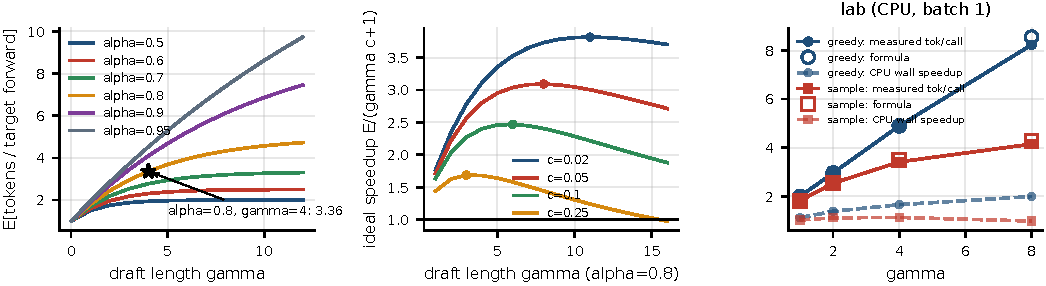
\includegraphics[width=\textwidth]{fig_speculative}
\caption{推测解码。左：式~\eqref{eq:spec} 的期望 token 数随草稿长度 $\gamma$ 和接受率 $\alpha$ 的变化，五角星是 $\alpha=0.8,\gamma=4$ 时的 3.36；$\alpha$ 越高，加长草稿越有用。
中：$\alpha=0.8$ 时理想加速比随 $\gamma$ 和草稿成本 $c$ 的变化，圆点是最优的 $\gamma$：草稿越贵，最优 $\gamma$ 越短，收益也越低。
右：本文配套实验（CS229S P2，CPU，batch 1）中每次目标调用实测得到的 token 数（实心）与公式（空心）相差不到 4\%，但 CPU 上的墙钟加速只有 0.98--1.99 倍。}
\label{fig:spec}
\end{figure*}

\begin{est}{$\alpha=0.8$、$\gamma=4$ 的推测解码}
$\mathbb{E}=(1-0.8^5)/(1-0.8)=(1-0.32768)/0.2\approx3.36$，即每次目标前向平均产出 3.36 个 token。如果草稿成本 $c=0.05$，$S=3.36/(4\times0.05+1)=3.36/1.2\approx2.8$。
从图~\ref{fig:spec} 中图可以读出，$c=0.05$ 时最优的 $\gamma$ 约为 8（$S\approx3.1$），$c=0.25$ 时最优 $\gamma$ 降到 3，$S$ 只有约 1.7。
\end{est}

\lab{CS229S P2}在一个合成语法上训练了 4 层的目标模型（79.7 万参数）和 1 层的草稿模型，实现了采样版的接受--拒绝和贪心版的推测解码，并用显式给出的 $p,q$ 做了 60,000 次试验来检验输出分布。
其中有三个结论值得在面试里讲。第一，贪心版的输出和目标模型逐 token 一致（16/16）。第二，$\alpha$ 的估计方法很容易出错：必须用「接受数 /（接受数 + 拒绝数）」；
如果用「接受数 / 提议数」，第一次拒绝之后那些从未被检验过的草稿也被算进了分母，$\gamma=8$ 时会把 0.80 算成 0.41。
第三，CPU 上验证 $\gamma+1$ 个 token 的一次前向是单 token 前向的 1.41--1.61 倍，草稿的相对成本 $c=0.256$，这是被调用开销抬高的结果，而不是参数比 0.04，
所以墙钟加速只有 0.98--1.99 倍。这个结果不能推出「GPU 上也只有 2 倍」：GPU 上 batch=1 的 decode 受带宽限制，多验证几个 token 几乎不增加时间。

也有方法不用独立的草稿模型。Medusa~\cite{cai2024medusa} 在目标模型上加几个解码头，并行预测后面的若干 token，再用树形 attention 一次验证多条候选；
EAGLE~\cite{li2024eagle} 在特征层（倒数第二层的隐状态）上自回归地生成草稿，接受率更高。但它们仍受同一条约束：只有当验证近乎免费，也就是 decode 受访存限制时，才划算。

\begin{qa}{推测解码为什么不改变输出分布？}
\ans 因为接受和重采样两条路径的概率加起来正好是 $p(x)$。对任意 token $x$，输出它的概率 $=q(x)\min(1,p(x)/q(x))+P(\text{拒绝})\cdot\frac{\max(0,p(x)-q(x))}{\sum_y\max(0,p(y)-q(y))}$。
第一项等于 $\min(p,q)$；拒绝的概率是 $1-\sum\min(p,q)=\sum\max(0,p-q)$，所以第二项等于 $\max(0,p-q)$。两项之和恰好是 $p(x)$。
贪心版则保证输出和目标模型的贪心解码完全相同。
\wrong 「草稿模型猜错的 token 会混进输出」；或者「推测解码是一种近似方法」。
\end{qa}

\begin{qa}{大 batch 下推测解码还划算吗？}
\ans 通常不划算。batch 越大，decode 越接近算力受限（7B 在 batch 512 时已经受算力限制），多验证的 $\gamma$ 个 token 就不再免费。
式~\eqref{eq:spec} 的分母变成 $\gamma c+v$，而 $v$ 会随 batch 增大逐渐接近 $\gamma+1$；同时，被拒绝的 token 白白浪费了算力。所以高吞吐的服务一般只在负载低时打开推测解码，
或者动态调整 $\gamma$。
\wrong 「推测解码在任何负载下都能加速」。
\end{qa}

\subsection{量化}

推测解码是让每次读权重多产出几个 token，量化则是直接减少要读的字节。线性量化把张量映射到 $b$ 位整数网格上。对称量化取 $\text{scale}=\max|x|/(2^{b-1}-1)$，$q=\mathrm{round}(x/\text{scale})$，
误差上界是 scale/2。粒度从粗到细分为 per-tensor、per-channel 和 per-group（$g=64/128$）。
LLM 量化的核心难点是激活离群值：少数固定通道的幅值比其他通道大几十到上百倍~\cite{dettmers2022llmint8}。per-tensor 的 scale 被它撑大以后，其余通道几乎都被量化成了 0。
表~\ref{tab:quant} 汇总了主要的应对方法。

\begin{table*}[!t]
\centering
\caption{LLM 量化方法对比（W$x$A$y$ 表示权重 $x$ 位、激活 $y$ 位）}
\label{tab:quant}
\footnotesize
\begin{tabularx}{\textwidth}{@{}l c L{3.4cm} Y Y@{}}
\toprule
方法 & 典型配置 & 核心思想 & 加速来源 & 代价与局限 \\
\midrule
LLM.int8()~\cite{dettmers2022llmint8} & W8A8 + FP16 离群 & 把幅值超阈值（6）的特征维拆出走 FP16，其余 INT8 & 显存减半 & 混合分解需额外 kernel，吞吐不一定提升 \\
SmoothQuant~\cite{xiao2023smoothquant} & W8A8 & $XW=(X\mathrm{diag}(s)^{-1})(\mathrm{diag}(s)W)$，把激活难度按通道挪到权重 & INT8 tensor core，prefill 与 decode 都受益 & 需要校准；权重也变难量化 \\
GPTQ~\cite{frantar2023gptq} & W4A16/W3A16 & 逐列量化，用 Hessian $H=X^\top X$ 的逆把舍入误差补偿到未量化的列 & decode 读权重字节减少 & 依赖校准数据的协方差；prefill 不加速 \\
AWQ~\cite{lin2024awq} & W4A16 & 按激活幅值找出约 1\% 的显著权重通道，用等价缩放保护 & 同上，硬件友好（无混合精度） & 需要校准；仍是 weight-only \\
QLoRA~\cite{dettmers2023qlora} & NF4 权重 + BF16 LoRA & 4 位 NormalFloat、双重量化、分页优化器 & 微调显存 & 训练吞吐低于 BF16 \\
FP8~\cite{micikevicius2022fp8} & W8A8（E4M3） & 浮点格式自带动态范围，per-tensor/per-block scale & H100 tensor core 2 倍算力 & 需要 scale 管理；仅新硬件支持 \\
\bottomrule
\end{tabularx}
\end{table*}

\begin{figure*}[!t]
\centering
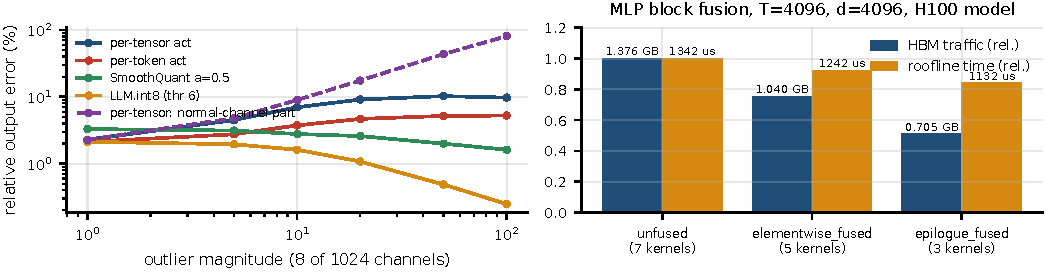
\includegraphics[width=\textwidth]{fig_lab_compress}
\caption{本文配套实验（15-849 编译与压缩）。左：在 1024 个通道中放入 8 个离群通道，W8A8（权重 per-channel）的相对输出误差随离群倍数的变化。
50 倍离群时，per-tensor 激活量化的误差是 10.2\%，per-token 是 5.17\%，SmoothQuant（$\alpha=0.5$）是 1.99\%，LLM.int8 是 0.49\%。虚线显示，per-tensor 下普通通道部分的误差高达 43.6\%（100 倍时 80.8\%）；
整体误差「只有」10\%，是因为离群通道同时主导了输出的范数，掩盖了普通通道的损坏。右：Transformer MLP 块的融合，HBM 流量 $-49\%$，roofline 时间却只有 $-16\%$（第~\ref{sec:kernel} 节）。数据是合成的，用于说明机制。}
\label{fig:labcompress}
\end{figure*}

\lab{15-849 编译与压缩}的激活量化结果见图~\ref{fig:labcompress}。权重量化方面还有两点值得一提。其一，对重尾（Student-$t$）分布的权重，INT8 per-tensor 的误差是 20.6\%，
per-channel 是 1.97\%，group128 是 1.11\%，说明整张表的步长是由一个极大值决定的。其二，GPTQ 只在输入之间有相关性时才有用：输入谱衰减为 1.0 时，测试误差是 3.5\%（RTN 是 25.3\%）；
输入各向同性时反而略差（28.2\% 对 26.4\%）。原因是 $H\approx cI$ 时没有可利用的相关性，补偿项拟合的只是校准集的采样噪声。

\begin{qa}{为什么 LLM 的激活难量化，权重容易？}
\ans 因为离群值集中在激活上。权重近似零均值，离群值少；激活却在少数固定通道上有几十到上百倍的离群值，per-tensor INT8 的 scale 被撑大，普通通道只剩下几个量化级。
离群值是按\emph{通道}出现的，而不是按 token，所以 per-token 量化只能缓解（配套实验中误差减半）。LLM.int8 把离群通道拆出去走 FP16；SmoothQuant 用逐通道缩放把激活的难度挪到权重上。
\wrong 「INT8 对所有张量都一样好做」。
\end{qa}

\begin{qa}{weight-only 量化（W4A16）为什么能加速 decode，却不一定加速 prefill？W4A16 与 W8A8 怎么选？}
\ans 因为两个阶段的瓶颈不同。decode 受带宽限制，读 INT4 权重比 BF16 少 4 倍字节，反量化在寄存器里做，计算本来就不是瓶颈；prefill 受算力限制，权重仍要反量化成 BF16 才能上 tensor core，
算力一点没省，反而多了反量化的开销。所以小 batch、低时延的 decode 选 W4A16；大 batch、prefill 占比高、受算力限制的服务选 W8A8 或 FP8，用上 INT8/FP8 的 tensor core。
\wrong 「量化总是更快」；「4 位一定比 8 位快」。
\end{qa}

\begin{table*}[!t]
\centering
\caption{LLM 服务系统的关键技术对比}
\label{tab:serving}
\footnotesize
\begin{tabularx}{\textwidth}{@{}l L{3.2cm} L{3.6cm} Y@{}}
\toprule
系统/技术 & 解决的问题 & 机制 & 代价与适用条件 \\
\midrule
Orca~\cite{yu2022orca} & 静态批处理的空等与排队 & iteration-level 调度、selective batching & 需要 KV 管理支持动态加入/离开 \\
vLLM~\cite{kwon2023vllm} & KV 碎片与预留浪费 & PagedAttention：块表、引用计数、CoW、抢占（swap/recompute） & kernel 间接寻址；块大小折中 \\
Sarathi-Serve~\cite{agrawal2024sarathi} & prefill 造成 decode 卡顿（TPOT 尖峰） & chunked prefill、stall-free batching、token 预算 & prefill 被切块后 TTFT 略增；预算需调 \\
DistServe~\cite{zhong2024distserve} / Splitwise~\cite{patel2024splitwise} & prefill 与 decode 干扰、并行配置耦合 & PD 分离、按 goodput 规划两池并行度 & KV 跨机传输；容量配比与运维 \\
SGLang~\cite{zheng2024sglang} & 请求间前缀重复计算；结构化程序 & RadixAttention 前缀缓存、缓存感知调度、约束解码 & 缓存占用显存；需要亲和路由 \\
推测解码~\cite{leviathan2023fast,cai2024medusa,li2024eagle} & batch 小时 decode 带宽受限 & 草稿 + 并行验证，分布无偏 & 大 batch 下收益消失；需要草稿模型或额外头 \\
S-LoRA~\cite{sheng2024slora} / Punica~\cite{chen2024punica} & 多 LoRA 适配器服务 & 统一分页、分段 gather-matmul（SGMV） & 异构 rank 的 kernel 效率 \\
\bottomrule
\end{tabularx}
\end{table*}

表~\ref{tab:serving} 把本节讨论过的服务技术放在一起。它们几乎都在应对同一个约束：decode 受带宽和 KV 容量限制，prefill 受算力限制，而在线服务又要同时满足 TTFT 和 TPOT。
面试中的系统设计题（比如上面的 70B 估算）考的就是能否按收益给这些技术排序。一个合理的顺序是：先上 continuous batching 和 PagedAttention，
再做量化和前缀缓存，然后是 chunked prefill 或 PD 分离，最后才是推测解码。

\begin{keypts}
\begin{itemize}
\item decode 步时 $\approx\max(2NB/P,\ (sN+\mathrm{KV})/\mathrm{BW})$；临界 batch 约等于拐点（H100 约 295），但 KV 不能被 batch 分摊。
\item KV $=2Ln_{kv}d_{\text{head}}TBs$：8B 是 128~KiB/token，70B 是 320~KiB/token；8B 在 8K 时 1~GiB，128K 时 16~GiB。
\item 调度的演进：continuous batching、PagedAttention、chunked prefill，再到 PD 分离和前缀缓存。
\item 推测解码 $\mathbb{E}=(1-\alpha^{\gamma+1})/(1-\alpha)$，$\alpha=0.8,\gamma=4$ 时为 3.36；输出分布无偏；大 batch 下不划算。
\item 激活离群值按通道出现；W4A16 加速 decode，W8A8/FP8 加速 prefill。
\end{itemize}
\end{keypts}

\begin{research}
\begin{itemize}
\item 本文的模拟显示，chunked prefill 的吞吐优势有一部分来自 roofline 假设下「混合步完美重叠」。真实 GPU 上混合步的效率是多少？
可以在真实引擎中固定 decode batch，改变捎带的 prefill token 数，测量步长时间与 $\max(F/P,B/\mathrm{BW})$ 的偏差。
\item 推测解码的接受率 $\alpha$ 并不是独立同分布的，它随位置、温度和领域变化。一个可做的实验是按位置统计接受率，检验式~\eqref{eq:spec} 的偏差，
并据此设计自适应 $\gamma$ 的策略。评估指标必须是同一负载下的 goodput，而不是 batch=1 时的加速比。
\end{itemize}
\end{research}
